
  \begin{figure}[t]
   \centering
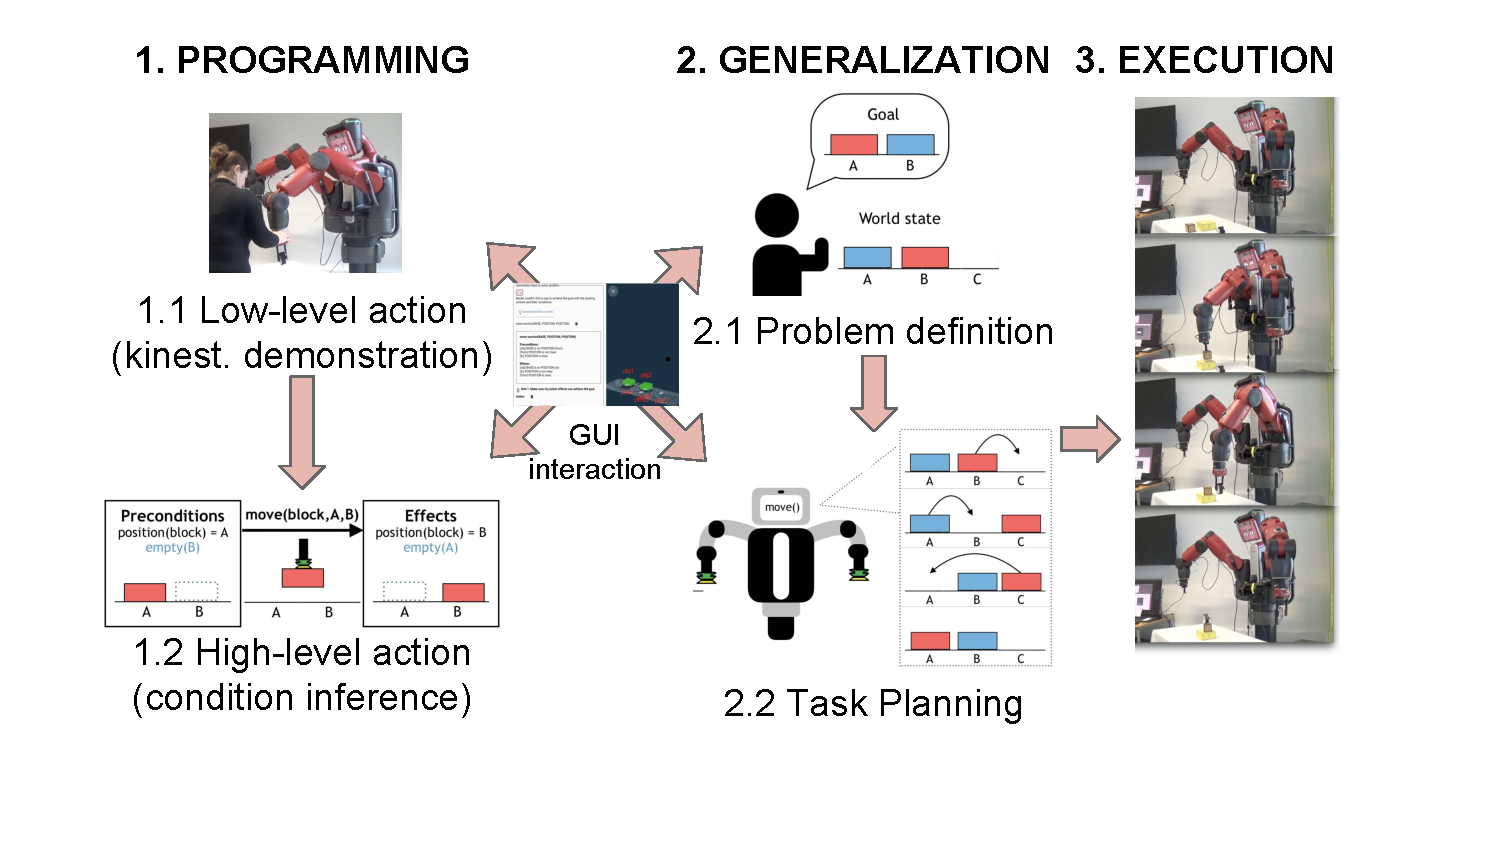
\includegraphics[width=0.7\linewidth]{figures/overview.pdf}
   \caption{Overview of iRoPro that allows users to teach low- and high-level actions by demonstration. The user interacts with the GUI to run the demonstration, modify inferred action conditions, create new planning problems for the robot to solve and execute.}
   \label{fig:overview}
  \end{figure}	
  \section{Approach}
\label{sec:approach}
Our approach aims at providing end-users with an intuitive way of teaching robots new actions that can be reused with a task planner to solve more complex tasks.
Given a single demonstration, the robot should learn both \textit{how} (\sect{sec:lowlevel}) and \textit{when} (\sect{sec:highlevel}) an action should be applied.
To accelerate the programming process, action conditions are directly inferred from a single demonstration (\sect{sec:inference}).
The action generalisation is performed on both low- and high-level representations (\sect{sec:generalisation}), allowing it to be reused with a task planner (\sect{sec:planning}).
We will describe our approach in the following sections.

\subsection{Low-level Action Representation}
\label{sec:lowlevel}
We represent low-level actions as proposed in previous work (\cite{akgun2012keyframe,alexandrova2014robot}), where the action is represented as a sparse sequence of gripper states (open/close) and end-effector poses relative to perceived objects or to the robot's coordinate frame.
For example, the pick-and-place action of an object to a marked position could be represented as poses relative to the object (for the pick action), poses relative to the target position (for the place action), and corresponding open/close gripper states. 

While these actions can be learned from multiple demonstrations (\cite{niekum2012learning}), we take the approach that only requires a single demonstration by heuristically assigning poses and letting the user correct them if needed (\cite{alexandrova2014robot}).
Thus, the first demonstrated action is already an executable action.
The user can teach multiple manipulation actions and discriminate between them by associating different conditions that specify \textit{when} the robot should use them (\eg actions using claw or suction grippers).
These conditions are discussed next in \sect{sec:highlevel}.

In iRoPro, new actions are initialised with the robot's end-effector poses in a neutral position (as seen in \fig{fig:dispositif}) to allow unobstructed object detection.
Action executions are performed by first detecting the landmarks in the environment, calculating the end-effector poses relative to the observed landmarks, and interpolating between the poses.

% \begin{figure}
% 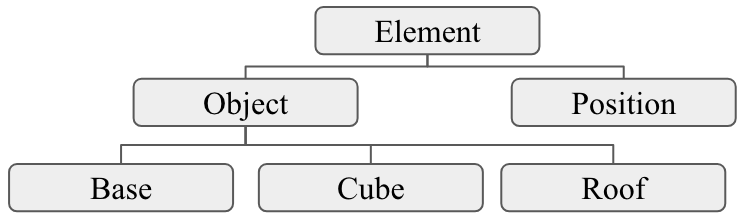
\includegraphics[width=0.8\linewidth]{figures/object-type-hierarchy.png}
% \caption{Type hierarchy describing a general type `Element' that includes `Object' and `Position' and three object types `Base', `Cube', and `Roof'.}
% \label{fig:type-hierarchy}
% \end{figure}


\subsection{High-level Action Representation}
\label{sec:highlevel}
We represent high-level actions as proposed in previous work on task planning (\cite{ghallab2004automated}), where an action is represented as a tuple $a = (\text{param}(a), \text{pre}(a),$ $\text{eff}(a))$, whose elements are:
\begin{itemize}
\item $\text{param}(a)$: set of parameters that $a$ applies to
\item $\text{pre}(a)$: set of predicates that must be true to apply $a$
\item $\text{eff}(a)^{-}$: set of predicates that are false after applying $a$
\item $\text{eff}(a)^{+}$: set of predicates that are true after applying $a$
\end{itemize}
where $\text{eff}(a) = \text{eff}(a)^{-} \cup \text{eff}(a)^{+}$. 
Action parameters are world instances that the robot interacts with and are associated with a \textit{type}.
For example, in iRoPro, we implemented a type hierarchy, consisting of a general type ELEMENT, divided into POSITION and OBJECT, which further divides into BASE, CUBE, and ROOF (\fig{fig:dispositif}).

Predicates are used to describe object states and relations between them and are defined in first-order logic.
In our graphical interface, predicates are translated from first-order logic (`on(obj, A)') to English statements (`obj is on A').
In iRoPro, we implemented predicates that are commonly used in task planning domains as well as two additional ones to describe object properties:
\begin{itemize}
    \item \textit{ELEMENT is clear}: an element has nothing on top of it
    \item \textit{OBJECT is on ELEMENT}: an object is on an element
    \item \textit{OBJECT is stackable on ELEMENT}: an object can be placed on an element
    \item \textit{OBJECT is flat}: an object has a flat top
    \item \textit{OBJECT is thin}: an object is thin
\end{itemize}
Note that the set of types and predicates could easily be extended for more complex tasks and that it is possible to detect them automatically.
However, this is beyond the scope of our work, so in our implementation CUBE and BASE objects are by default flat, while CUBE and ROOF objects are thin enough for the robot to grasp.
% \begin{tabular}{rl} \hline
% & \textbf{move(obj1, A, B):}\\ \hline
% Param: & obj1 - object, A - position, B - position\\
% Pre: & obj1 is on A, B is clear \\
% Eff$^{+}$: & obj1 is on B, A is clear\\
% Eff$^{-}$: & obj1 is not on B, B is not clear\\
%  & \\
% \end{tabular}

%An example of a move action of an object from position A to B is shown in \fig{fig:action-model}.
%Action conditions can be learned from multiple demonstrations (\citet{abdo2013learning}).
%We take an approach where the action can be learned from a single demonstration by inferring parameters, preconditions, and effects from observed states.
%We will discuss this in the next section.

\begin{figure}
\centering
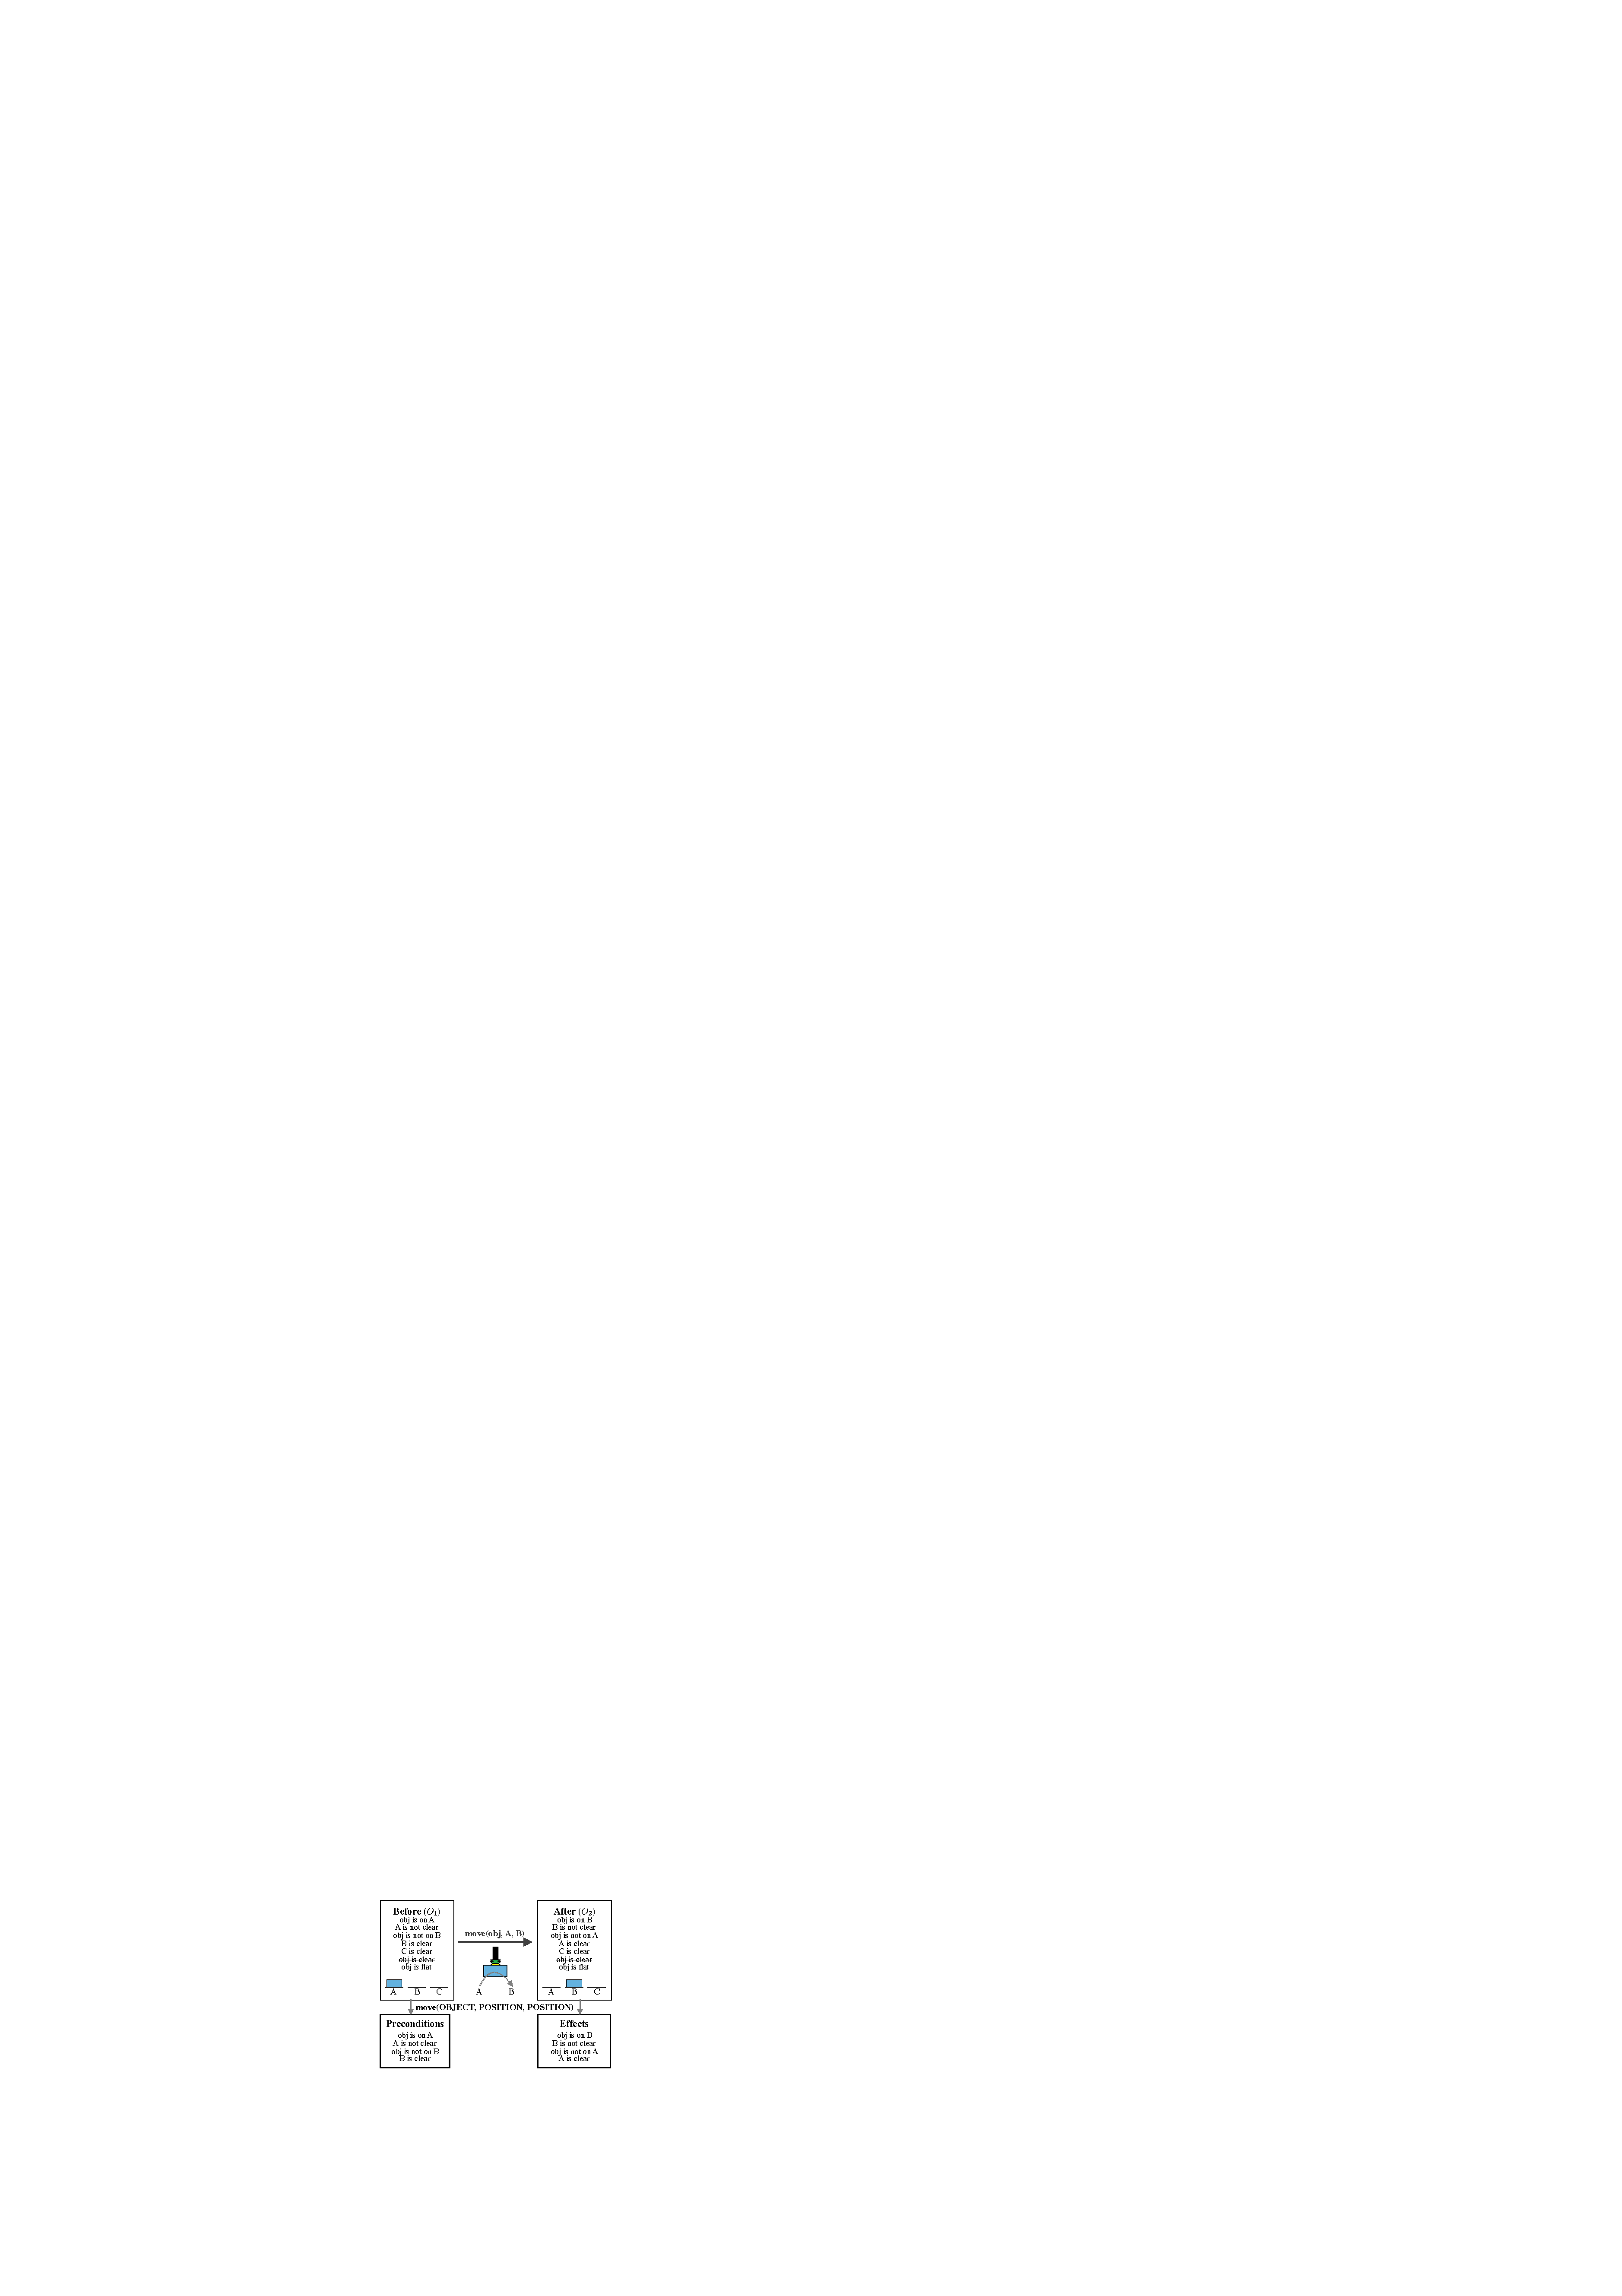
\includegraphics[width=0.5\linewidth]{figures/high-level.pdf}
\caption{Example of a high-level action for moving an object from A to B. Conditions are inferred from the observed predicates before ($O_1$) and after ($O_2$) the demonstration.
}
\label{fig:action-model}
\end{figure}

\subsection{Action Inference from Demonstration}
\label{sec:inference}
Instead of manually defining action parameters, preconditions, and effects, we accelerate the programming process by inferring them from the observed sensor data during the teaching phase.
Object types are inferred based on their detected bounding boxes (see \sect{sec:implementation}).
Object positions are determined by the proximity of the object to given positions.
If the nearest position \emph{p} to the object \emph{o} is within a certain threshold $d$, then the predicates `\emph{o} is on \emph{p}' and `\emph{p} is not clear' are added to the detected world state.

To infer the action conditions, the robot perceives the initial world state   before %(\textit{precondition})
and after the kinesthetic action demonstration as seen in similar work for learning object manipulation tasks (\cite{ahmadzadeh2015learning}).
%(\textit{effects}).
Let $O_1 = \{\phi_1, \phi_2, ... \}$ be the set of predicates observed before the action demonstration and $O_2 = \{\psi_1, \psi_2, ... \}$ after.
The action inference is the heuristic deduction of predicates that have changed between $O_1$ and $O_2$, \ie
\begin{align*} \text{pre}(a) = \{\phi_i | \phi_i \in O_1 \wedge \phi_i \notin O_2 \}, \\
\text{eff}(a) = \{\psi_i | \psi_i \notin O_1 \wedge \psi_i \in O_2 \}, 
\end{align*}
where $\text{eff}(a)$ includes positive and negative effects (\fig{fig:action-model}).

A predicate $\phi$ has variables $\text{var}(\phi) = \{v_1, v_2, \dots\}$, where each $v_i$ has a type.
Therefore, action parameters are the set of variables that appear in either preconditions or effects, \ie
\begin{align*}
     \text{param}(a) = \{v_i &| \hspace{0.3cm}\exists \phi \in \text{pre}(a) \text{ s.t. } v_i \in \text{var}(\phi)\\
     &\lor \exists \psi \in \text{eff}(a) \text{ s.t. } v_i \in \text{var}(\psi) \}
\end{align*}
%where $type(p_i) = type(v_i)$.
%First infer the positions, then state that all other elements must be clear

Note that conditions could be learned from multiple demonstrations (\cite{abdo2013learning,konidaris2018fromSkills}).
Our work argues for accelerating the teaching phase by learning from a single demonstration and letting the user act as the expert to correct wrongly inferred conditions.

 
\subsection{Action Generalisation}
\label{sec:generalisation}
Due to simultaneously learning low- and high-level action representations, an action is generalised in two ways:

1. Low-level: the demonstrated action consists of poses relative to detected landmarks during the action demonstration (\sect{sec:lowlevel}). 
To generalise this action to different landmarks, objects are redetected and relative poses are re-calculated.

2. High-level: the action parameter types and preconditions specify what landmarks an action can be applied to. 
Changing these properties via the GUI allows an action to be generalised and the taught manipulation action to be transferred to other tasks.


\subsection{Task Planning}
\label{sec:planning}
Task planners are used to generate solutions, or action sequences, to solve complex problems.
%ught actions are reused with existing task planners by translating them into PDDL (\citet{mcdermott1998pddl}). 
Given a description of a planning \textit{domain}, \ie object types, actions with preconditions and effects, we can define a planning \textit{problem} with an initial state and a desired goal state. 
The planner generates an optimal action sequence, or \textit{plan}, which guarantees the transition from initial state to the goal state. 
PDDL (\cite{mcdermott1998pddl}) %extends the STRIPS \cite{fikes1971strips} formalism and 
is often used as a standard encoding language for planning problems.
%as it allows type structures
A move action as shown in \fig{fig:action-model} is defined as follows:

\begin{verbatim}
(:action move
 :parameters (?obj - object 
              ?A - position ?B - position)
 :precondition (and (on ?obj ?A)(clear ?B)
            not(on ?obj ?B) not(clear ?A))
 :effect (and (on ?obj ?B) (clear ?A)
            not(on ?obj ?A) not(clear ?B))
\end{verbatim}

A planning problem consists of an initial state and a goal state and can only be solved using existing actions in the domain.
For example, the problem of swapping two objects obj1, obj2 on A and B respectively with C unoccupied, can be defined as:
\begin{verbatim}
(:objects obj1 obj2 - object
          A B C - position)
(:init (and (on obj1 A) (on obj2 B) 
        (clear C)))
(:goal (and (on obj1 B) (on obj2 A)))
\end{verbatim}
The planner would generate the following action sequence:
\begin{verbatim}
1. move(obj1, A, C)
2. move(obj2, B, A)
3. move(obj1, C, B)
\end{verbatim}
An example of a complete planning domain and problem in PDDL can be found in the attached materials.

\begin{figure}[t]
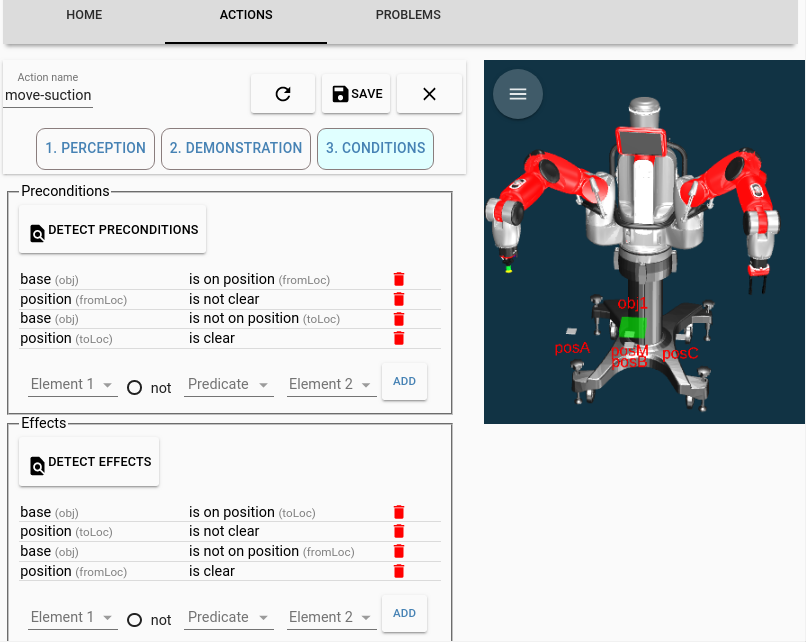
\includegraphics[width=\linewidth]{figures/gui.png}
    \caption{The iRoPro interface showing the action condition menu and an interactive visualisation of the Baxter robot and detected objects.}\label{fig:gui-action-3}%
\end{figure}

\begin{figure*}[t]
\centering
 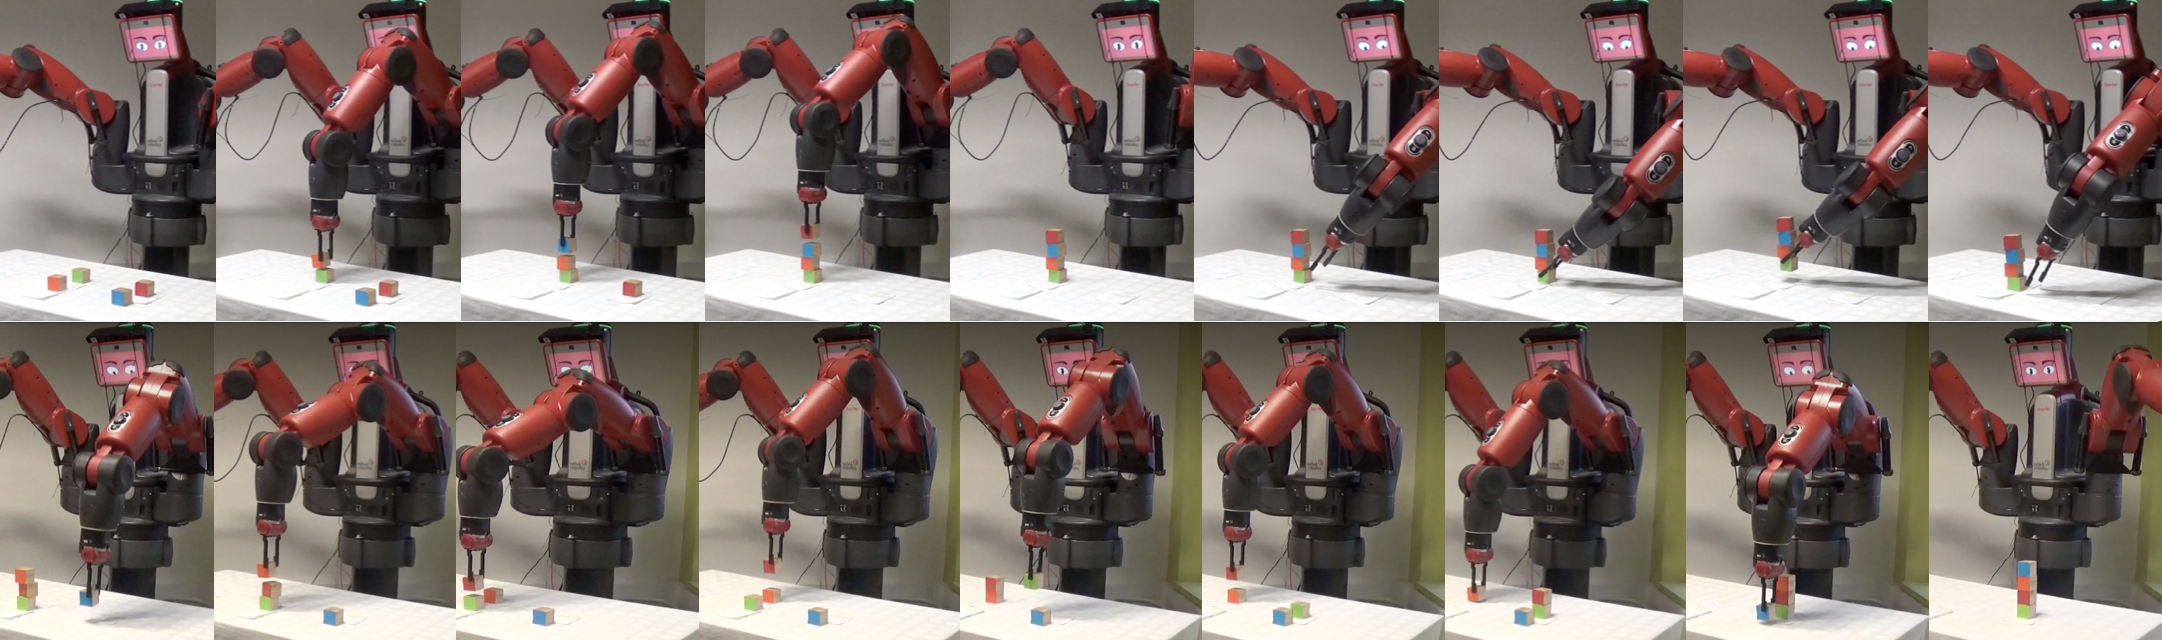
\includegraphics[width=\linewidth]{figures/filmstrip.png}
\caption{Snapshots from the executions of the system evaluation (Tasks 3\&4) showing a claw grip from top and side.}
\label{fig:filmstrip}
\end{figure*}
\section{System}
\label{sec:system}
\subsection{Platform}
\label{sec:platform}
We implemented our system on a Baxter robot with two arms (one claw and one suction gripper), both with 7-DoF and a load capacity of 2.2kg each.
For the object perception we mounted a Kinect Xbox 360 depth camera on the robot.
We developed a user interface as a web application that can be accessed via a browser on a PC, tablet or smartphone.

The source code for iRoPro is developed in ROS (\cite{quigley2009ros}) and available online\footnote{Blinded for review}. %ysl208/rapid\_pbd}.
The low-level action is learned using the open-source system Rapid PbD\footnote{https://github.com/jstnhuang/rapid\_pbd}.
%for teaching actions by keyframe-based demonstration.
The integration of the task planner is implemented using the ROS package PDDL planner\footnote{http://docs.ros.org/indigo/api/pddl\_planner}.

\subsection{Implementation Details}
\label{sec:implementation}
In our implementation, landmarks are either predefined table positions or 
objects that are detected from Kinect point cloud clusters using an open-source tabletop segmentation library\footnote{https://github.com/jstnhuang/surface\_perception}.
An object is represented by its detected location and bounding box $obj = (x,y,z, width, length, height)$, where the bounding box is used to infer the object type (\sect{sec:inference}).

We implemented a partial PDDL domain in iRoPro that includes a set of predefined object types and predicates (\sect{sec:highlevel}).
The user completes the domain by creating new actions and uses the integrated task planner to solve new problems.

% To that end, the user mainly interacts with the system for two main aspects: Actions and Problems.
% We will discuss them in the following sections.

\subsection{Interactive Robot Programming}
\label{sec:interactive}
The user interacts with the GUI (\fig{fig:gui-action-3}) to visualise the robot and the detected objects, create new actions, run the kinesthetic teaching by demonstration, correct inferred action parameters or conditions, create and solve new problems with the task planner.
The interactive robot programming cycle consists of creating and modifying actions and problems.
\subsubsection{Actions} New actions are taught by kinesthetically moving the robot's arms (low-level action) and assigning action conditions (high-level action).
The low-level action is learned %using the open-source system Rapid PbD for teaching actions 
by keyframe-based demonstration (\sect{sec:lowlevel}).
To verify the taught action, the user can have the robot re-execute it immediately.
The high-level action is inferred by capturing the world state before and after the action demonstration (as described in \sect{sec:inference}).
Action generalisation can be done by modifying action properties (\sect{sec:generalisation}).
To teach more actions, the user can either create a new one or copy a previously taught action and modify it.
\subsubsection{Problems} New planning problems can be created if at least one action exists.
To create a problem, the robot first detects the existing landmarks and infers their types and initial states.
The user can modify them if the inference was not correct.
Then, the user enters predicates that describe the goal state to achieve.
The complete planning domain and problem are translated into PDDL and sent to the Fast-Forward planner (\cite{hoffmann2001ff}).
If a solution is found that reaches the goal, it is displayed on the GUI for the user to verify and execute on the robot.
If no solution is found or if the generated plan is wrong, the user can open a debug menu which summarises the entire planning domain with hints described in natural language to investigate the problem (\eg `make sure the action effects can achieve the goal states').
In our user study (\sect{sec:quanteval}) we found that this helped users understand how the system worked and why the generated plan was wrong.
Once the user modified actions, initial or goal states, they can relaunch the planner to see if a correct plan is generated.
To solve new tasks, the user can create a new problem or modify existing ones by redetecting the objects.

\subsection{Plan Execution} 
The generated plan is a sequence of actions with parameters that correspond to detected objects.
For each action, the sequence of end-effector poses are calculated relative to the landmarks that the action is being applied to (\sect{sec:lowlevel}).
To accelerate the execution, we only detect the landmarks once at the start and save their new positions in a mental model.
After each action execution, the user can confirm that it executed correctly and the mental model is updated with the latest positions of the changed landmarks.
The mental model is also used as a workaround for our limited perception system for problems with stacked objects in their initial states (\sect{sec:discussions}).

%\paragraph{Reusable Actions} 
%Our system allows the robot to reuse previously taught actions for unseen problems with different objects and types.
%The user is only required to teach the robot simple atomic actions and the robot reuses them for complex tasks that require multiple subactions.
%Without having to explicitly teach the robot the action sequence, the robot can solve any user-defined goal autonomously using the planner.
%To address new tasks and problems, the user can simply change problem parameters or action conditions if the programmed manipulation action can be transferred.

% steps for using the system are:
% \begin{enumerate}
%     \item Create a new planning domain
%     \item {Create new actions
%     \begin{enumerate}
%         \item Detect landmarks (parameters and types)
%         \item Kinesthetic demonstration of action
%         \item Assign conditions (preconditions/effects)
%     \end{enumerate}}
%     \item {Create new planning problem
%     \begin{enumerate}
%         \item Detect landmarks (initial state)
%         \item Assign goal state
%         \item Verify generated plan and execute
%     \end{enumerate}}
% \end{enumerate}


% \subsection{Teaching Strategies}
% \label{sec:strategies}
% \todo {either create one action and try to generalise it as much as possible by changing parameter types and adding preconditions, or copy an action to have the same manipulation action but change the parameters for other specific tasks. 
% As creating an action from scratch takes the longest, it is most optimal to reuse demonstrated manipulation actions.}